% CVPR 2025 Paper Template; see https://github.com/cvpr-org/author-kit

\documentclass[10pt,twocolumn,letterpaper]{article}

%%%%%%%%% PAPER TYPE  - PLEASE UPDATE FOR FINAL VERSION
\usepackage{cvpr}              % To produce the CAMERA-READY version
% \usepackage[review]{cvpr}      % To produce the REVIEW version
% \usepackage[pagenumbers]{cvpr} % To force page numbers, e.g. for an arXiv version

% Import additional packages in the preamble file, before hyperref
\input{preamble}


% (Or just hit 'q' on the first LaTeX run, let it finish, and you should be clear).
\definecolor{cvprblue}{rgb}{0.21,0.49,0.74}
\usepackage[pagebackref,breaklinks,colorlinks,allcolors=cvprblue]{hyperref}

\usepackage{multirow} % for multi-row tables
\usepackage{tabularx}
\usepackage{pifont}  % for symboles

% Required packages in preamble
\usepackage{amsmath}
\usepackage{xcolor}
\usepackage{mathtools}

% Define custom colors
\definecolor{sumcolor}{RGB}{70,130,180}   % Steel Blue
\definecolor{gradcolor}{RGB}{178,34,34}   % Firebrick Red
\definecolor{normcolor}{RGB}{34,139,34}   % Forest Green

% Required packages in preamble
\usepackage{amsmath}
\usepackage{xcolor}
\usepackage{mathtools}
\usepackage{tcolorbox}
\usepackage{empheq}
% \usepackage{multicol} % for \columnbreak

% Define custom colors
\definecolor{sumcolor}{RGB}{70,130,180}    % Steel Blue
\definecolor{gradcolor}{RGB}{178,34,34}    % Firebrick Red
\definecolor{normcolor}{RGB}{34,139,34}    % Forest Green
\definecolor{boxcolor1}{RGB}{230,230,250}  % Lavender
\definecolor{boxcolor2}{RGB}{255,240,245}  % Lavender Blush
\definecolor{boxcolor3}{RGB}{230,245,230}  % Lavender Blush

% Define custom boxes
\newcommand{\highlight}[2][boxcolor1]{%
  \colorbox{#1}{$\displaystyle#2$}}

% From LeGrad
\usepackage{xcolor, colortbl}
\definecolor{almond}{RGB}{186,210,225}
\newcommand{\tabbold}{\fontseries{b}\selectfont}

%%%%%%%%% PAPER ID  - PLEASE UPDATE
\def\paperID{16303} % *** Enter the Paper ID here
\def\confName{CVPR}
\def\confYear{2025}

%%%%%%%%% TITLE - PLEASE UPDATE
\title{LeGrad:
An Explainability Method for Vision Transformers via Feature Formation Sensitivity}


%%%%%%%%% AUTHORS - PLEASE UPDATE
\author{%
    Walid Bousselham$^{1}$ \quad
    Angie Boggust$^2$  \quad
    Sofian Chaybouti$^{1}$ \quad
    Hendrik Strobelt$^{3, 4}$  \quad
    Hilde Kuehne$^{1, 3}$ \\
    \kern-1.1em\small{
    $^1$University of Bonn \& Goethe University Frankfurt,
    $^2$MIT CSAIL, 
    $^3$MIT-IBM Watson AI Lab
    $^4$IBM Research, 
    } \\
}

% \author{First Author\\
% Institution1\\
% Institution1 address\\
% {\tt\small firstauthor@i1.org}
% % For a paper whose authors are all at the same institution,
% % omit the following lines up until the closing ``}''.
% % Additional authors and addresses can be added with ``\and'',
% % just like the second author.
% % To save space, use either the email address or home page, not both
% \and
% Second Author\\
% Institution2\\
% First line of institution2 address\\
% {\tt\small secondauthor@i2.org}
% }

% \author{Walid Bousselham\inst{1,2} \and
%  Angie Boggust\inst{3} \and
% Sofian Chaybouti \inst{1,2} \and \\
% Hendrik Strobelt \inst{4, 5} \and
% Hilde Kuehne \inst{1,2,4}
% }
% \institute{
% University of Bonn \and Goethe University Frankfurt \and
% MIT CSAIL \and
% MIT-IBM Watson AI Lab\and
% IBM Research}

\begin{document}
\maketitle


\begin{abstract}
% %\vspace{-3em}
Vision Transformers (ViTs) have become a standard architecture in computer vision. However, because of their modeling of long-range dependencies through self-attention mechanisms, the explainability of these models remains a challenge. % can still be improved
To address this, we propose LeGrad, an explainability method specifically designed for ViTs. 
LeGrad computes the gradient with respect to the attention maps of single ViT layers, considering the gradient itself as the explainability signal.
We aggregate the signal over all layers, combining the activations of the last as well as intermediate tokens to produce the merged explainability map.
This makes LeGrad a conceptually simple and an easy-to-implement method to enhance the transparency of ViTs. 
We evaluate LeGrad in various setups, including segmentation, perturbation, and open-vocabulary settings, showcasing its improved spatial fidelity as well as its versatility compared to other SotA explainability methods.% and robustness to perturbations.
\end{abstract}

\begin{figure*}[h]
    \vspace{-1em}
    \centering
    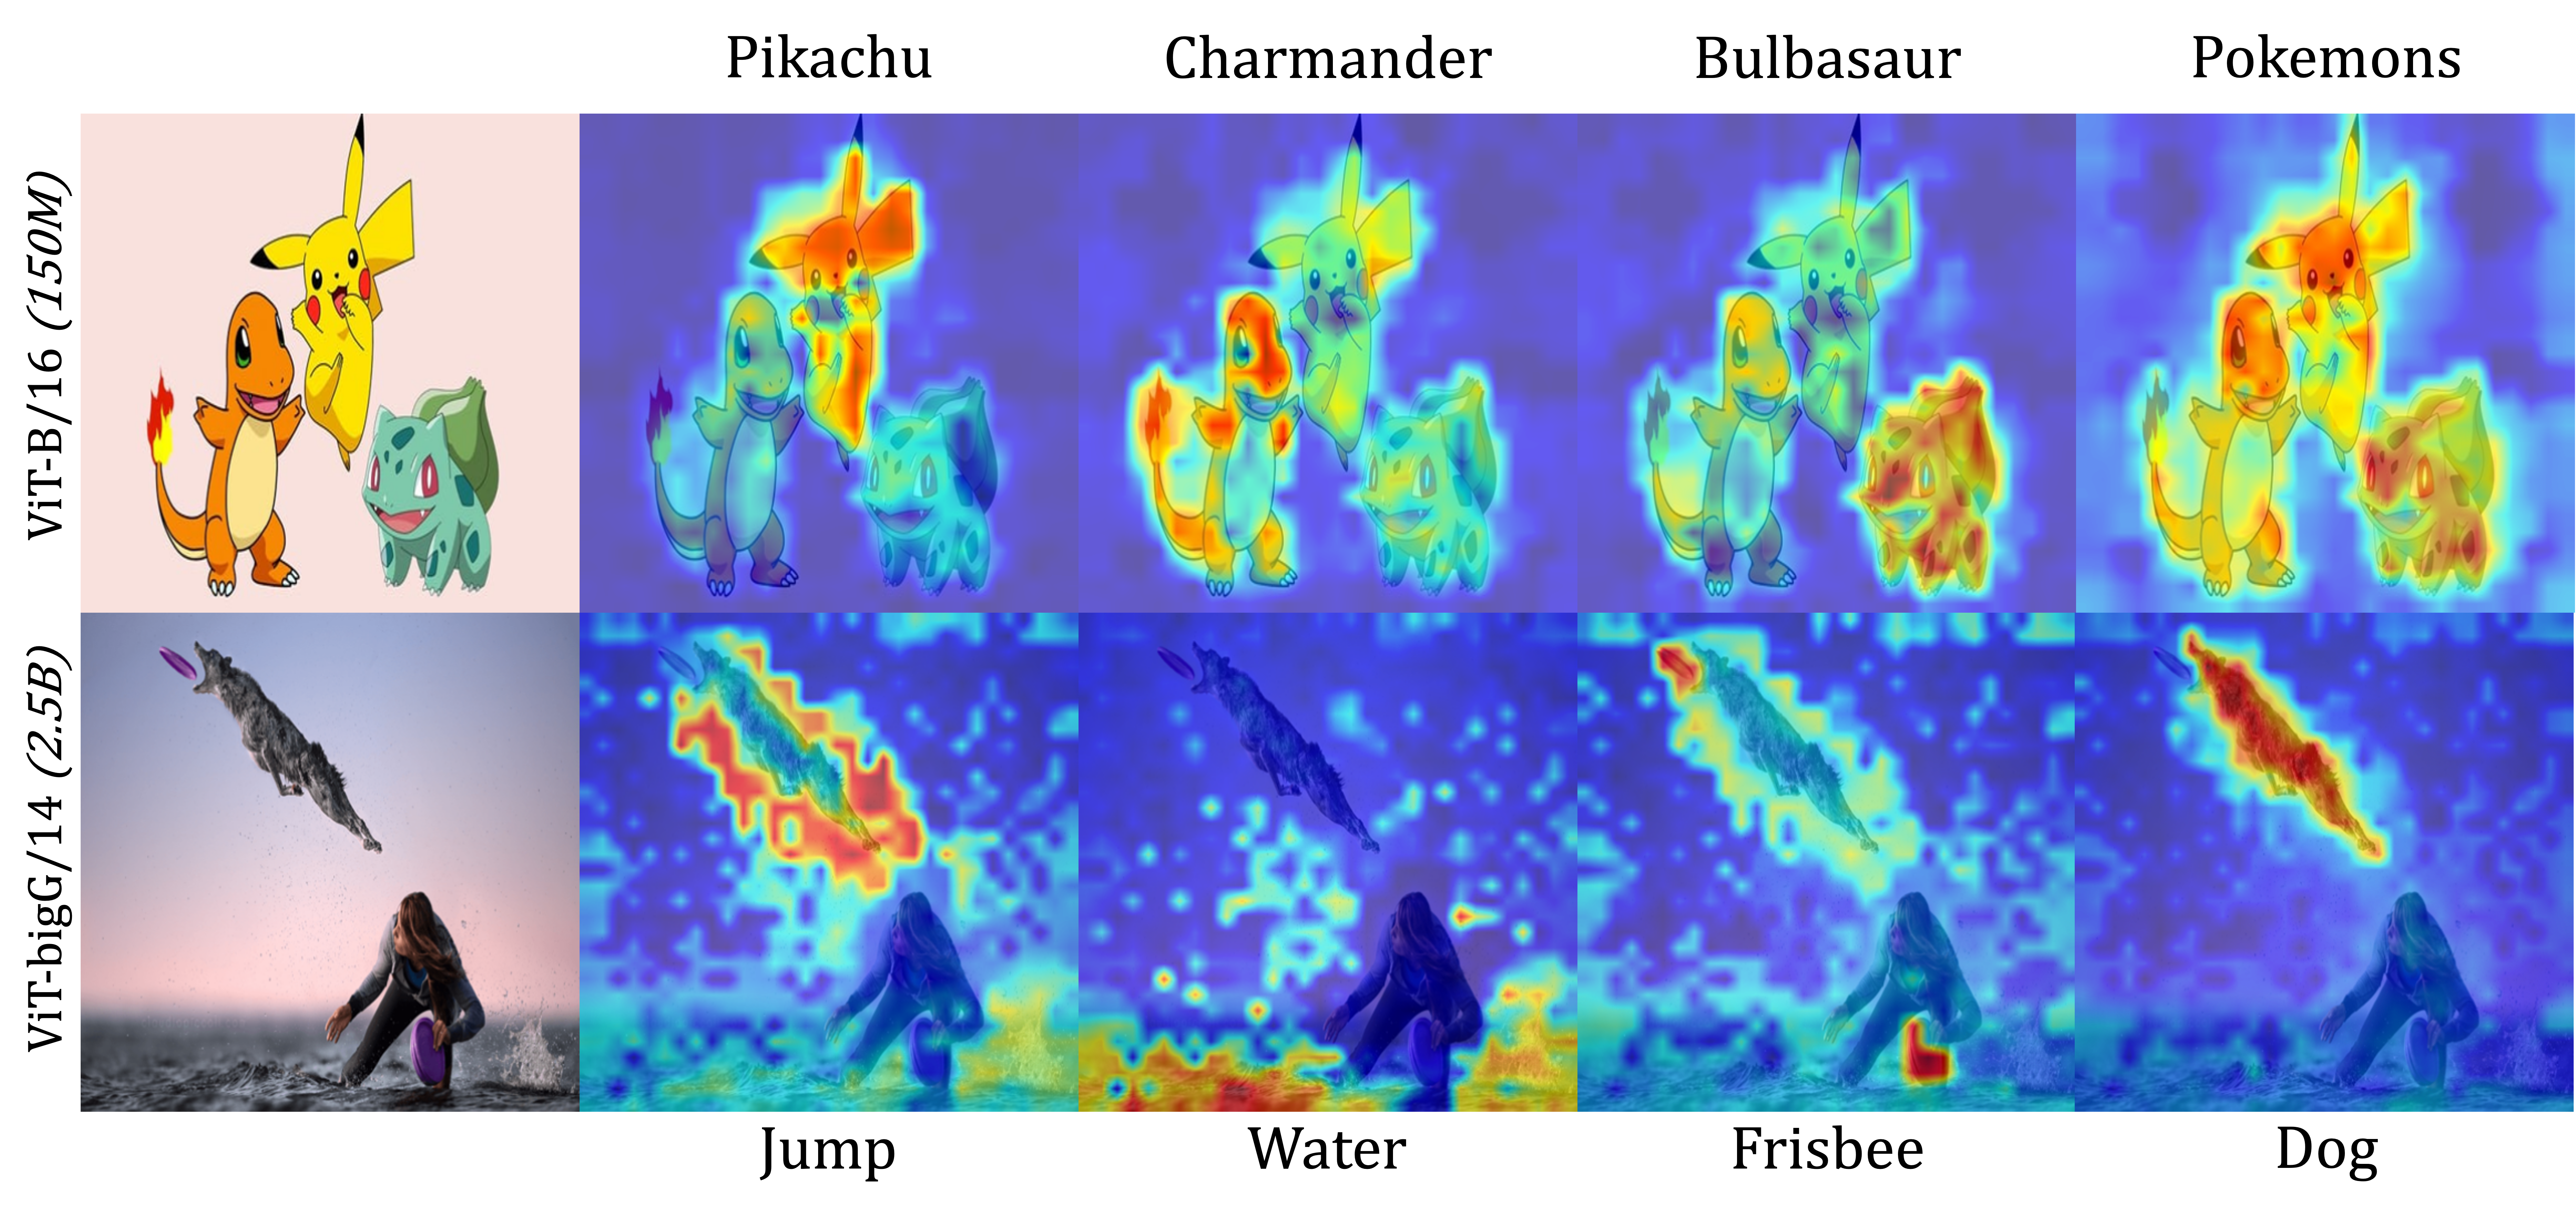
\includegraphics[width=.9\textwidth]{images/teaser_figure_longer.pdf}
    \vspace{-1.5em}
    \caption{\textbf{LeGrad explainability maps:} For a given VLM and an input textual prompt, LeGrad generates a heatmap indicating the part of the image that is most sensitive to that prompt. Examples shown for OpenCLIP ViT-B/16(150M params.) and ViT-bigG/14(2B params.).}
    \label{fig:teaser_figure}
    \vspace{-1.5em}
\end{figure*}

\section{Introduction}
\label{sec:intro}



Vision Transformers (ViTs)\citep{dosovitskiy2020image} have significantly influcened the field of computer vision with their ability to model long-range dependencies through self-attention mechanisms. %~\citep{touvron2021training, liu2021swin, xie2021segformer, arnab2021vivit, peebles2023scalable}. %
But explanability methods designed for convolutional or feed-forward neural networks are not directly applicable to ViTs due to their architectural requirements, like GradCAM's~\citep{selvaraju2017grad} reliance on convolutional layers and Layer-wise Relevance Propagation's (LRP)~\citep{bach2015pixel} specific layer-wise propagation rules.
While ViT-specific explainability techniques exist, including adaptations of traditional methods~\citep{chefer2020transformer, selvaraju2017grad,chefer2021generic}, attention-based techniques~\citep{abnar2020quantifying, voita2019analyzing,chefer2020transformer,chefer2021generic}, and text-based explanations~\citep{hernandez2021natural,goh2021multimodal,abnar2020quantifying}, the explainability those architectures remains a challenge. 


To address this problem, we propose \textbf{LeGrad}, a \textbf{L}ayerwise \textbf{E}xplainability method that considers the \textbf{Grad}ient with respect to the attention maps. LeGrad is specifically designed for ViTs as it leverages the self-attention mechanism to generate relevancy maps highlighting the most influential parts of an image for the model's prediction.
Compared to other methods, LeGrad uses the gradient with respect to the attention maps as the explanatory signal, as e.g. opposed to CheferCam~\citep{chefer2020transformer,chefer2021generic}, which uses the gradient to weight the attention maps. This is done independently for each layer. The final explainability signal is then pooled over all layers of the ViT. Note that using a layerwise gradient, compared to other signals, allows to sum up over different layers without further need for normalization. To further improve the signal, the gradient is clipped by a ReLU function preventing negative gradients to impact positive activations (see Figure~\ref{fig:method_figure} for details).
The approach is conceptually simple and versatile, as it only requires the gradient w.r.t. to the ViT's attention maps. This facilitates its adoption across various applications and architecture, including larger ViTs such as ViT-BigG as well as attention pooling architectures~\citep{lee2019set, zhai2023sigmoid}.  %enhancing the transparency of ViTs. 

% We evaluate the proposed method for various ViT backbones
% on four challenging tasks: segmentation, open-vocabulary detection, and perturbation and audio localization on ImageNet~\citep{russakovsky2015imagenet, gao2022luss}, OpenImagesV7~\citep{benenson2022colouring} as well as ADE20KSound/SpeechPrompted\citep{hamilton2024separating} . It shows that while current methods struggle especially with the diverse object categories in OpenImagesV7, LeGrad can achieve performance gains of $2\times$--$5\times$, reaching a score of $48.4$ \textit{p-mIoU} on OpenImagesV7 using OpenCLIP-ViT-B/16. Furthermore, we demonstrate the applicability of LeGrad to very large models, such as the ViT-BigG/14~\citep{cherti2023reproducible} with 2.5 billion parameters. Finally, it also adapts well to different feature aggregation strategies employed by ViTs~\citep{radford2021learning, zhai2023sigmoid}, making it a versatile tool for explainability. LeGrad also establishes a new SoTA on zero-shoot sound localization on ADE10KSoundPrompted by scoring $+15mAP$/$+14mIoU$ over previous SoTA.

We evaluate the proposed method for various ViT backbones
on four challenging tasks, segmentation, open-vocabulary detection, perturbation, and audio localization, spanning over various datasets, incl. ImageNet~\citep{russakovsky2015imagenet, gao2022luss}, OpenImagesV7~\citep{benenson2022colouring}, and ADE20KSound/SpeechPrompted~\citep{hamilton2024separating}. It shows that while current methods struggle with the diverse object categories in OpenImagesV7, LeGrad reaches a score of $48.4$ \textit{p-mIoU} on OpenImagesV7 using OpenCLIP-ViT-B/16. Furthermore, we demonstrate the applicability of LeGrad to very large models, such as the ViT-BigG/14~\citep{cherti2023reproducible} with 2.5 billion parameters while also adapting well to different feature aggregation strategies employed e.g. by SigLIP~\citep{zhai2023sigmoid}. Finally, LeGrad also establishes a new SoTA on zero-shot sound localization on ADE20KSoundPrompted scoring $+14mIoU$ over previous SoTA.


We summarize the contributions as follows: 
(1) We propose LeGrad as a layerwise explainability method based on the gradient with respect to ViTs attention maps. 
(2) As the layerwise explainability allows to easily pool over many layers, LeGrad scales to large architectures such as ViT-BigG/14 and is applicable to various feature aggregation methods.
(3) We evaluate LeGrad on various tasks and benchmarks, showing its improvement compared to other state-of-the-art explainability methods especially for large-scale open vocabulary settings. 

% --------------------------------------------------
% --------------------------------------------------
% \begin{figure*}[t]
%     \centering
%     \includegraphics[width=1.\textwidth]{images/method_figure.pdf}
%     %\vspace{-2.5em}
%     \caption{\textbf{Overview of LeGrad:} Given a text prompt or a classifier $\mathcal{C}$, an activation $s^l$ is computed for each layer $l$. The activation $s^l$ is then used to compute the explainability map of that layer. The layerwise explainability maps are then merged to produce LeGrad's output.}
%     \label{fig:method_figure}
% \end{figure*}
% %\vspace{-1em}
% 
\section{Related Work}
% 
\textbf{Gradient-Based Explanation Methods}
Feature-attribution methods are a commonly used explanation technique that explains model decisions by assigning a score to each image pixel, representing its importance to the model's output.
Generally, these methods can be categorized into two groups~\citep{molnar2019}\,---\,gradient-based methods that compute explanations based on the gradient of the prediction of the model with respect to each input pixel~\citep{simonyan2013deep,erhan2009visualizing,sundararajan2017axiomatic, springenberg2014striving,smilkov2017smoothgrad,kapishnikov2019xrai,selvaraju2017grad} and perturbation-based methods that measure pixel importance by successively perturbing the input images and measuring the impact on the model output~\citep{lundberg2017unified,ribeiro2016should,petsiuk2018rise,carter2019made,zeiler2014visualizing}.
While both types of methods have been used successfully to identify correlations and trustworthiness in traditional computer vision models~\citep{boggust2022shared, carter2021overinterpretation}, gradient-based methods are often more computationally efficient since they only require a single backwards pass. Further, they are easy to interpret since they are a direct function of the model's parameters and do not rely on additional models or image modifications.
However, many existing gradient-based methods were designed for convolutional and feed-forward architectures, so it is non-trivial to directly apply them to ViTs since ViTs do not contain spatial feature maps and include complex interactions between patches induced by the self-attention mechanism.
%Instead, we build on the simplicity and computational efficiency of gradient-based explanation methods to develop LeGrad, a gradient-based feature-attribution method specifically designed for ViT architectures.
\begin{figure*}[t]
    \centering
    \vspace{-0.5em}
    \includegraphics[width=1.\textwidth]{images/method_figure.pdf}
    \vspace{-2.5em}
    \caption{\textbf{Overview of LeGrad:} Given a text prompt or a classifier $\mathcal{C}$, an activation $s^l$ is computed for each layer $l$. The activation $s^l$ is then used to compute the explainability map of that layer. The layerwise explainability maps are then merged to produce LeGrad's output.}
    \vspace{-1em}
    \label{fig:method_figure}
\end{figure*}
%
As most gradient-based methods were designed prior to the widespread use of ViTs, researchers have recently made efforts to adapt existing methods and to develop new ones specifically for transformers.
Chefer et al.~\citep{chefer2020transformer} extend LRP~\citep{bach2015pixel} to transformers by integrating gradients within the self-attention layers. 
However, this approach is computationally heavy and is inflexible to architecture changes as it requires specific implementation for each module of the network.
To circumvent that complexity, CheferCAM~\citep{chefer2021generic} weights the attention by their gradient and aggregates it through the layer via matrix multiplication.
However, the use of gradients to weigh the attention heads' importance makes this method class-specific.
%LeGrad on the other hand is class-agnostic and computationally efficient, making it simple to use and more effective than these other methods (see \cref{sec:experiments} for a quantitative evaluation).



\noindent\textbf{Explanability Methods for ViT}
A separate line of research has proposed using ViT attention maps, as opposed to gradients, as a way to explain for transformers' decisions~\citep{abnar2020quantifying, voita2019analyzing}. 
One attention-based method, rollout~\citep{abnar2020quantifying}, traces the flow of importance through the transformer's layers by linearly combining the attention maps via matrix multiplication.
Attention flow~\citep{abnar2020quantifying} contextualizes the attention mechanism as a max-flow problem; however, it is computationally demanding and has not been extensively evaluated for vision tasks.
While these methods offer insights into the attention mechanism, they often neglect the non-linear interactions between attention heads and the subsequent layers. 
Moreover, they may not adequately distinguish between positive and negative contributions to the final decision, leading to potentially misleading interpretations, as found in Chefer et al.~\citep{chefer2020transformer}. 
Compared to that LeGrad uses the gradient w.r.t. to the attention maps, thereby assessing the sensitivity of the attention maps to a change in the patch tokens. 
%LeGrad does not attempt to track the flow of information throughout the transformer layers but, rather, focuses on assessing the sensitivity of the model prediction at each layer for every location of the image.
%While LeGrad also focuses on the attention maps to generate its explanation, it uses the gradient w.r.t. to the attention maps, thereby assessing the sensitivity of the attention maps to a change in the patch tokens. 
%LeGrad does not attempt to track the flow of information throughout the transformer layers but, rather, focuses on assessing the sensitivity of the model prediction at each layer for every location of the image.


\noindent\textbf{Vision-Language Explainability Methods}
Research has also explored vision-langauge models for interpreting representations in vision models. 
For instance, leveraging CLIP's language-image space, researchers have provided text descriptions for active neuron regions~\citep{hernandez2021natural, goh2021multimodal} and projected model features into text-based concept banks~\citep{gandelsman2023interpreting}. 
In particular, \textsc{TextSpan}~\citep{gandelsman2023interpreting} focuses on the explainability of CLIP-like models. 
It refrains from using gradient computation by aggregating the intermediate features' similarities along a given text direction, creating a relevancy map for a text query. 
LeGrad advances this line of work by focusing on the sensitivity of feature representations within ViTs to generate relevancy maps that can be adapted to various feature aggregation strategies.

% \textbf{Evaluating Explanation Methods}
% As the popularity of feature-attribution based explanation methods has grown, so has research evaluating their ability to faithfully reflect the model's decision making process~\citep{sundararajan2017axiomatic,yeh2019on,kindermans2019reliability,samek2016evaluating,hooker2019benchmark,alvarez2018on,adebayo2018sanity,tomsett2020sanity,gomez2022metrics,zhang2016top}.
% Faithfulness is an important criteria because explanation methods that highlight human-salient pixels may look correct even if the model relies on spurious correlations and give human interpreters unwarranted confidence in the model.
% These evaluations can be categorized based on the aspect of faithfulness that they test~\citep{boggust2023saliency}, such as the method's sensitivity to meaningful changes to the input, model, or data~\citep{sundararajan2017axiomatic,yeh2019on,kindermans2019reliability,samek2016evaluating,hooker2019benchmark,alvarez2018on,adebayo2018sanity,tomsett2020sanity} and its ability to highlight a succinct and meaningful pixel region~\citep{gomez2022metrics,zhang2016top}.
% We evaluate LeGrad on both of these types of tests, demonstrating that it is faithful to the model's decision making process by testing that removing LeGrad's important pixels impacts the model's output and checking that LeGrad's output corresponds to a concise object region. %



% --------------------------------------------------
\section{Method}
In this section, we first introduce ViT's mechanics and the different feature aggregation mechanisms used for this architecture.
We then explain the details of LeGrad, starting by a single layer and then extending it to multiple layers.



\subsection{Background: Feature formation in ViTs}\label{sec:method:subsec:feature_formation}

The ViT architecture is a sequence-based model that processes images by dividing them into a grid of $n$ patches. These patches are linearly embedded and concatenated with a class token $z_0^0 = z^0_{[CLS]} \in \mathbb{R}^d$, which is designed to capture the global image representation for classification tasks. The input image $I$ is thus represented as a sequence of $n+1$ tokens $Z^0 = \{z_0^0, z_1^0, \dots, z_n^0\}$, each of dimension $d$, with positional encodings added to retain spatial information. 

The transformation of the initial sequence $Z^0 \in \mathbb{R}^{(n+1) \times d}$ through the ViT involves $L$ layers, each performing a series of operations. Specifically, each layer $l$ applies multi-head self-attention (MSA) followed by a multilayer perceptron (MLP) block, both with residual connections:
\begin{equation}
% \begin{aligned}
\hat{Z}^l = \text{MSA}^l(Z^{l-1}) + Z^{l-1}, \quad
Z^l = \text{MLP}^l(\hat{Z}^l) + \hat{Z}^l.
% \end{aligned}
\end{equation}

% \noindent After $L$ layers, the image representation can be obtained via:% various strategies:
 After $L$ layers, the visual features can be obtained via:% various strategies:

\noindent \textbf{[CLS] token:} The class token approach, as introduced in ViT~\citep{dosovitskiy2020image}, uses the processed class token as the image embedding $\bar{z}_{[CLS]} = z^L_0$. This method relies on the transformer's ability to aggregate information from the patch tokens into the class token during training.


\noindent \textbf{Attentional Pooler:} Attention Pooling, as e.g. used in SigLIP~\citep{zhai2023sigmoid} employs an multi-head attention layer~\citep{lee2019set, yu2022coca} with a learnable query token $q_{pool} \in \mathbb{R}^d$. This token interacts with the final layer patch tokens to produce the pooled representation $\bar{z}_{AttnPool}$:
\begin{equation}
\bar{z}_{AttnPool} = \text{softmax}\left( \frac{q_{pool} \cdot (W_KZ^L)^T}{\sqrt{d}} \right) (W_V Z^L),
\end{equation}
where $W_K, W_V \in \mathbb{R}^{d \times d}$ are learnable projection matrices.

Independent of the feature aggregation strategy, it is important for an explainability method to account for the iterative nature of feature formation in ViTs and to capture the contributions of all layers for the final representation. 
LeGrad addresses this by fusing information from each layer, allowing for both, a granular as well as a joint, holistic interpretation of the model’s predictions.

\subsection{Explainability Method: LeGrad}\label{sec:method:subsec:LeGrad}

We denote the output tokens of each block $l$ of the ViT as $Z^l = \{ z_0^l, z_1^l, \dots, z_n^l \} \in \mathbb{R}^{(n+1) \times d}$, where %
 $d$ is the dimensionality of each token, and $ \bar{z}^l$ is the average over the tokens of the respective layer $l$, defined as $ \bar{z}^l = \frac{1}{n+1} \sum_{i=0}^n z_i^l$ .

% C as a mapping
Consider a mapping model $\mathcal{C} \in \mathbb{R}^{d \times C}$, that maps the token dimension $d$ to $C$ logits. 
This classifier can be learned during training for a supervised classification task (e.g., ImageNet) and in that case $C$ is the number of classes. Or it can be formed from text embeddings of some prompts in the case of zero-shot classifier, \textit{e.g.,} vision-language models like CLIP, then $C$ is the number of prompts.
For a given layer $l$, the mapping model $\mathcal{C}$ then generates a prediction $\bar{y}^l$, which can be the output of the classifier or, in case of vision-language models, the vector of results of dot products of the text and image embeddings. 
% Consider a classifier $\mathcal{C} \in \mathbb{R}^{d \times C}$, where $C$ is the number of classes. This classifier can be learned during training for a supervised classification task (e.g., ImageNet) or can be formed from text embeddings of class descriptions for a zero-shot classifier, as in the case of vision-language models like CLIP, generating a prediction $\bar{y}$. 
This prediction $\bar{y}^l$ is obtained by passing the aggregated feature representation of the ViT, noted $\bar{z}^l$, through the mapping $\mathcal{C}$: 
\vspace{-0.5em}
\begin{equation}
\bar{y}^l = \bar{z}^l \cdot \mathcal{C} \in \mathbb{R}^C.
\vspace{-0.5em}
\end{equation}
%
Note that most explainability methods only use the final outputs of the model. We argue that also leveraging intermediate representations is beneficial (see Section~\ref{subsec:layer_abl}).
% whereas here we also leverage intermediate representation (see section for ablation).
%
The following we first describe how to obtain the explainability map for a single layer, using an arbitrary layer $l$ as an example and then generalize it to multiple layers. The overall method is visualized Figure~\ref{fig:method_figure}.

\begin{figure}
    \centering
    \vspace{-2em}
    \includegraphics[width=0.4\textwidth]{images/layer_method.pdf}
    \vspace{-1em}
    \caption{\textbf{LeGrad} for a single layer.}
    \label{fig:method_single_layer}
    \vspace{-1em}
\end{figure}
\textbf{Process for a Single Layer:} To compute a 2D map that highlights the image regions most influential for the model's prediction of a particular class, we focus on the activation with respect to the target class/prompt $\hat{c}$, denoted by $s^l = \bar{y}^l_{[\hat{c}]}$. The attention operation within a ViT is key to information sharing, and thus our method concentrates on this process.
% 
We compute the gradient of the activation $s^l$ with respect to the attention map of layer $l$, as shown in Figure~\ref{fig:method_single_layer}, denoted as $\mathbf{A}^l \in \mathbb{R}^{h \times n \times n}$:
\begin{equation}
\nabla \mathbf{A}^l = \frac{\partial s}{\partial \mathbf{A}^l} \in \mathbb{R}^{h \times (n+1) \times (n+1)},
\end{equation}
where $h$ is the number of heads in the self-attention operation. Negative gradients are discarded by a ReLU function (noted $(.)^+$), and the gradient is averaged across the patch and head dimensions:
\begin{equation}
\hat{E^l}(s) = \frac{1}{h \cdot (n+1)} \sum_h \sum_i \left( \nabla \mathbf{A}^l_{h, i, .} \right)^+ \in \mathbb{R}^{n+1}.
\end{equation}

To obtain the final explainability map, the column corresponding to the [CLS] token is removed, only considering the patch tokens, reshaped into a 2D map, and a min-max normalization is applied:
\begin{equation}
E^l(s) = \text{norm}(\text{reshape}(\hat{E}^{l}(s)_{1:})) \in \mathbb{R}^{W \times H}.
\end{equation}

\textbf{Process for Multiple Layers:} Recognizing that information aggregation occurs over several layers, we extend the process to all layers. For each layer $l$, we calculate the activation score $s^l$ using the intermediate tokens $Z^l$ and derive the explainability map accordingly:
\begin{equation}
\hat{E}^l(s^l) = \frac{1}{h \cdot (n+1)} \sum_h \sum_i \left( \nabla \mathbf{A}^l_{h, i, .} \right)^+ \in \mathbb{R}^{n+1}.
\end{equation}

We then average the explainability maps from each layer:
\begin{equation}\label{eq:aggregation}
\begin{aligned}
\bar{\mathbf{E}} &= \frac{1}{L} \sum_l \hat{E}^l(s^l)_{1:}
\end{aligned}
\end{equation}

And finally we reshape to the original image size and apply min-max normalization:
% Prior to normalization, we average the explainability maps from each layer:
\begin{equation}\label{eq:norm_and_reshap}
\begin{aligned}
\mathbf{E} &= \text{norm}(\text{reshape}(\bar{\mathbf{E}})) \in R^{W \times H}.
\end{aligned}
\end{equation}

This queries each patch token at a given layer about its influence on the prediction at that stage.


\textbf{Adaptation to Attentional Pooler:} For ViTs using an attentional pooler (\textit{e.g.} SigLIP~\citep{zhai2023sigmoid}), a slight modification is made to compute the activation $s^l$ at each layer. We apply the attentional pooler module $Attn_{pool}$ to each intermediate representation $Z^l$ to obtain a pooled query $q^l \in \mathbb{R}^d$. The activation $s^l$ with respect to the desired class $c$ is then computed as $s^l = q^l \cdot \mathcal{C}_{:,c} \in \mathbb{R}$. Instead of considering the self-attention map, we use the attention map of the attentional pooler, denoted $\mathbf{A}_{pool} \in \mathbb{R}^{h \times 1 \times n}$. Thus, for every layer $l$, $\nabla A^l = \frac{\partial s^l}{\partial A^l_{pool}}$.




% --------------------------------------------------

\section{Experiments}
\label{sec:experiments}

\subsection{Object Segmentation}
Following standard benchmarks~\citep{chefer2020transformer, chefer2021generic, gandelsman2023interpreting} we evaluate the ability of explainability methods to accurately localize an object in the image. $\diamondsuit$\textit{\textbf{Task:}}  To do so, we generate image heatmaps based on the activation of the groundtruth class for models trained with a classifier or based on the the class descriptions \textit{"A photo of a [class]"} for vision-language models. Subsequently, we apply a threshold to binarize these heatmaps (using a threshold of 0.5), thereby obtaining a foreground/background segmentation.$\diamondsuit$\textit{\textbf{Metric:}} We assess the quality of this segmentation by computing the mIoU (mean Intersection over Union), pixel accuracy and the mAP (mean Average Precision) zero-shot segmentations produced by different explainability methods. This benchmark serves as a testbed for evaluating the spatial fidelity of the methods.
$\diamondsuit$\textbf{Dataset:} In our evaluation of heatmap-based explainability methods, we adhere to a standardized protocol and use the ImageNet-Segmentation dataset~\citep{gao2022luss}, with $4,276$ images that provide segmentation annotations. 

Table \ref{tab:segmentation} compares LeGrad as well as other methods in the context of image segmentation using the ImageNet-segmentation dataset. LeGrad achieved a mIoU of 58.7\%, surpassing other SOTA explainability methods. Notably, it outperformed CheferCAM as a gradient-based method for ViTs, and TextSpan as a non-gradient-based method, indicating its robustness in capturing relevant image features for classification tasks.


% ----------------- Table Object Segmentation + Open-Vocabulary
\begin{table*}[t]
\vspace{-0.5em}
% =Table 1
\begin{minipage}{.3\linewidth} %
      \centering
      \vspace{-5.9mm}
         \begin{tabular}{lccc}
\toprule 
Method  & Pixel Acc.$\uparrow$ & mIoU$\uparrow$ & mAP$\uparrow$ \\ 
\midrule 
LRP & 52.81 & 33.57 & 54.37 \\
Partial-LRP & 61.49 & 40.71 & 72.29 \\
rollout & 60.63 & 40.64 & 74.47 \\
Raw attention & 65.67 & 43.83 & 76.05 \\
GradCAM & 70.27 & 44.50 & 70.30 \\
CheferCAM & 69.21 & 47.47 & 78.29 \\
TextSpan & 73.01 & 40.26 & 81.4 \\
\midrule 
\cellcolor{almond}LeGrad &  \cellcolor{almond} \textbf{77.52} & \cellcolor{almond} \textbf{58.66} & \cellcolor{almond} \textbf{82.49} \\
\bottomrule
\end{tabular}
\begin{minipage}{1.39\linewidth}
\caption{\textbf{Object Segmentation:} method on ImageNet-S using an OpenCLIP(ViT-B/16) model trained on Laion2B. 
}\label{tab:segmentation}
\end{minipage}
\end{minipage}%
%\quad \quad %\vspace{-0em}
% \hspace{10mm}
\hfill \hspace{8mm}
% \vspace{+2em}
%  ========== Table 2
\begin{minipage}{.3\linewidth} %
      \centering
        \begin{tabular}{lrrr}
\toprule 
& \multicolumn{3}{c}{p-mIoU $\uparrow$} \\
Method & B/16 & L/14 & H/14 \\ 
\midrule 
rollout & 8.75 & 6.85 & 5.82 \\
Raw attention & 0.94 & 1.60 & 0.85 \\
GradCAM & 8.72 & 2.80 & 2.46 \\
AttentionCAM & 5.87 & 4.74 & 1.20 \\
CheferCAM & 5.87 & 2.51 & 9.49 \\
TextSpan & 9.44 & 21.73 & 23.74 \\
\midrule 
\cellcolor{almond}LeGrad & \cellcolor{almond} \tabbold {48.38} & \cellcolor{almond} \tabbold {47.69} & \cellcolor{almond} \tabbold {46.51} \\
\bottomrule
\end{tabular} 
\vspace{+0.7em}
\begin{minipage}{1.18\linewidth}
\caption{\textbf{Open-Vocabulary Segmentation:}
methods comparison on OpenImagesV7 using different OpenCLIP model sizes.}
\label{tab:openvocabulary}
\end{minipage}
\end{minipage}  %
\vspace{-1.em}
\hfill
% ========= Table 3
\begin{minipage}{.2\linewidth}
    \centering
    \vspace{0.94em}
\resizebox{1\columnwidth}{!}{
    \begin{tabular}{l |l}
    \toprule 
       \multirow{2}{*}{Method} & \multirow{2}{*}{fps}\\
       \\
        \hline

    AttentionCAM & $103$\\
    GradCAM & $108$\\
    CheferCAM & $21$\\
    LRP & $4.0$\\
    TextSpan & $3.8$\\
    \hline
    \rowcolor{almond}LeGrad & $96$\\
    \bottomrule
    \end{tabular}
    }
    \caption{Inference speed comparison for ViT-B/16.}
    \label{tab:run_times}
    \end{minipage}
\end{table*}
% ----------------- End: Table Object Segmentation + Open-Vocabulary

\subsection{Open-Vocabulary localization}
For vision-language models, we extend our evaluation to encompass open-vocabulary scenarios by generating explainability maps for arbitrary text descriptions.
This allows us to assess the quality of explainability methods beyond the common classes found in ImageNet. 
$\diamondsuit$\textit{\textbf{Task:}} We generate a heatmap for each class object present in the image, binarize them (using a threshold of 0.5) and assess the localization accuracy.
$\diamondsuit$\textbf{Dataset/Metric:} We use OpenImageV7 dataset~\citep{benenson2022colouring}, which offers annotations for a diverse array of images depicting a broad spectrum of objects and scenarios. Following~\citep{bousselham2023grounding}, our evaluation utilizes the point-wise annotations of the validation set, which contains 36,702 images labeled with 5,827 unique class labels. Each image is associated with both positive and negative point annotations for the objects present. In our analysis, we focus exclusively on the classes that are actually depicted in each image.

 Table \ref{tab:openvocabulary} evaluates the performance on OpenImagesV7, testing the capabilities of all methods in handling diverse object categories. Note that for GradCAM we searched over the layers and took the one that was performing the best. LeGrad outperforms all other SOTA methods, with performance gains ranging from $2\times$ to $5\times$ compared to the second-best performing method. This can be seen as an indicator for LeGrad's capacity for fine-grained recognition. %

% ------------------ Audio Localization + inference speed
\begin{table*}[]
\begin{minipage}{.55\linewidth} %
%\vspace{+.9em}
\centering
\resizebox{1.\columnwidth}{!}{
\begin{tabular}{lrrrr|r}
\toprule 
& \multicolumn{4}{c}{ImageNet} & OpenImagesV7\\
& \multicolumn{2}{c}{Negative} & \multicolumn{2}{c}{Positive} & \\
Method & Predicted $\uparrow$ & Target $\uparrow$ & Predicted $\downarrow$& Target $\downarrow$ & p-mIoU $\uparrow$\\ 
\midrule 
rollout & 47.81 & 47.81 & 25.74 & 25.74& 0.07\\
Raw attention & 44.42 & 44.42 & 25.85 & 25.85& 0.09\\
GradCAM & 41.25 & 44.42 & 35.10 & 33.50 & 6.97\\
AttentionCAM & 45.62 & 45.71 & 45.01 & 44.92 & 0.19\\
CheferCAM & 47.12 & 49.13 & 22.35 & 21.15 & 1.94 \\
\cellcolor{almond} LeGrad & \cellcolor{almond} \tabbold 50.08 & \cellcolor{almond} \tabbold 51.67 & \cellcolor{almond} \tabbold 18.48 & \cellcolor{almond} \tabbold 17.55 & \cellcolor{almond} \tabbold 25.40\\
\bottomrule
\end{tabular}
}
\caption{\textbf{SOTA comparison on SigLIP-B/16:} Comparison of explainability methods on perturbation-based tasks on ImageNet-val and open-vocabulary localization on OpenImagesV7.}
\label{tab:pert_siglip}
\end{minipage} 
\hfill
\begin{minipage}{.4\linewidth} %
% \hspace{-4em}
    %\vspace{+0.5em}
    \centering
\resizebox{1\columnwidth}{!}{
\begin{tabular}{lrr|rr}
\toprule 
\multirow{2}{*}{Method}& \multicolumn{2}{c}{Speech Seg.} & \multicolumn{2}{c}{Sound Seg.}\\
& mAP$\uparrow$ & mIoU$\uparrow$  & mAP$\uparrow$ & mIoU$\uparrow$ \\
\midrule 
DAVENet & 32.2 & 26.3 & 16.8 & 17.0 \\
CAVMAE & 27.2 & 19.9 & 26.0 & 20.5 \\
 ImageBind & 20.2 & 19.7 & 18.3 & 18.1 \\ \hline
\rowcolor{almond} ImageBind + LeGrad & \tabbold 23.3 & \tabbold 21.8 &  \tabbold  48.0 & \tabbold 38.9 \\ \midrule
\color{gray} DenseAV* & \color{gray} \tabbold 48.7 & \color{gray} \tabbold 36.8 & \color{gray} 32.7 & \color{gray} 24.2 \\
\bottomrule
\end{tabular}
}
\caption{\textbf{Speech \& Sound prompted semantic segmentation:} Comparison of the sound localization methods on ADE20K Speech \& Sound Prompted dataset~\citep{hamilton2024separating}.}\label{tab:sound_localization}
    \end{minipage}
\vspace{-2em}
\end{table*} 
% ------------------ End: Audio Localization + inference speed

%\vspace{-1em}
\subsection{Audio Localization}
To further validate LeGrad versatility, we measure its ability to be used with audio-visual models. We use ImageBind\citep{girdhar2023imagebind}, a model trained to align several modality with the same image encoder, in particular the audio modality. We choose this model as it is widely used and the image encoder is a vanilla ViT, hence compatible with LeGrad.
$\diamondsuit$\textit{\textbf{Task:}} Given an audio prompt, we generate a heatmap that localize the part of the image that correspond to that audio. $\diamondsuit$\textit{\textbf{Dataset/Metric:}} We use the recently proposed ADE20kSoundPrompted and ADE20kSpeechPrompted\citep{hamilton2024separating} to measure the audio localization of ImageBind + LeGrad. Following~\citep{hamilton2024separating}, we report the mean Average Precision (\textit{mAP}) and the mean Intersection over Union (\textit{mIoU}) computed using the ground truth.

Table~\ref{tab:sound_localization} compares the sound localization performance of different state-of-the-art methods. We observe that when applied to the ImageBind model~\citep{girdhar2023imagebind}, LeGrad leads to a significant increase in sound segmentation performance, hence establishing a new SOTA on that benchmark by outperforming DAVENet~\citep{harwath2018jointly}, CAVMAE~\citep{gongcontrastive} and the previous SOTA DenseAV~\citep{hamilton2024separating}. The less pronounced improvement of LeGrad over ImageBind on speech segmentation is due to the fact that ImageBind was not trained with speech data (only sound). Therefore, since ImageBind performs poorly on speech, LeGrad cannot improve the localization further.




\subsection{Perturbation-Based Evaluation}\label{sec:exp:subsec:perturbation}
Next, to measure LeGrad's ability to faithfully identify features important to the model, we employ a perturbation-based methodology. $\diamondsuit$\textit{\textbf{Task:}} Given a classification dataset, we begin by generating explainability maps for every image using the different explainability methods. The analysis then consists of two complementary perturbation tests: positive and negative. In the positive perturbation test, image regions are occluded in descending order of their attributed relevance, as indicated by the explainability maps.
Conversely, the negative perturbation test occludes regions in ascending order of relevance (see the \textit{Annex} for more details and visualizations of positive/negative perturbations).
$\diamondsuit$\textit{\textbf{Metric:}} For both perturbation scenarios, we quantify the impact on the model's accuracy by computing the area under the curve (AUC) for pixel erasure, which ranges from 0\% to 90\%. This metric provides insight into the relationship between the relevance of image regions and the model's performance. The tests are applicable to both the predicted and ground-truth classes, with the expectation that class-specific methods will show improved performance in the latter. This dual perturbation approach enables a comprehensive evaluation of the network's explainability by highlighting the importance of specific image regions in the context of the model's classification accuracy.
$\diamondsuit$\textbf{Dataset:} Following common practices\cite{chefer2020transformer,chefer2021generic}, we use the ImageNet-val, which contains $50K$ images and covers $1,000$ classes.

\noindent As detailed in Table \ref{tab:perturbations}, LeGrad's performance is here comparable to TextSpan for positive perturbations and slightly superior for negative perturbations. For all other methods, LeGrad outperformes both attention-based (e.g., "rollout" and "raw attention") and gradient-based methods (e.g., GradCAM, AttentionCAM, and CheferCAM) across various model sizes and for both predicted and ground truth classes, emphasizing its ability to identify and preserve critical image regions for accurate classification.


\subsection{Speed Comparison} 
Table \ref{tab:run_times} compares the inference speed for different methods averaged over $1,000$ images. Generally, gradient-based methods are faster than methods like LRP and TextSpan. More specifically, despite using several layers for its prediction, LeGrads speed only drops slightly compared to GradCAM and AttentionCAM, which both use a single layer and are significantly faster than CheferCAM. The speed difference stems from summing the contribution of each layer rather than using matrix multiplication as in CheferCAM.


\subsection{Performance  on SigLIP}
We also evaluate the adaptability regarding the performance on SigLIP-B/16, a Vision-Language model employing an attentional pooler as shown in Table~\ref{tab:pert_siglip}. 
The results underscore the methods performance across both negative and positive perturbation-based benchmarks. Notably, in the open-vocabulary benchmark on OpenImagesV7, LeGrad achieved a p-mIoU of 25.4, significantly surpassing GradCAM's 7.0 p-mIoU, the next best method. 
These findings affirm the versatility of LeGrad, demonstrating its robust applicability to various pooling mechanisms within Vision Transformers. 
Further details on the methodological adaptations of LeGrad and other evaluated methods for compatibility with SigLIP are provided in the annex.



\begin{table*}[t]
\centering
\resizebox{1\columnwidth}{!}{
\begin{tabular}{llrr c rr}
\toprule 
& & \multicolumn{2}{c}{Negative} && \multicolumn{2}{c}{Positive} \\
 & Method & Pred. $\uparrow$ & Targ. $\uparrow$ && Pred. $\downarrow$& Targ. $\downarrow$\\ 
\midrule 
\multirow{7}{*}{\rotatebox[origin=c]{90}{ViT-B/16}} &rollout & 44.36& 44.36 && 23.03 &  23.03\\
&Raw attention & 46.97 &46.97 && 20.23 & 20.23 \\
&GradCAM &32.01 & 45.26 && 36.52 &  22.86\\
&AttentionCAM & 39.56& 39.68 && 34.28 &  34.12\\
&CheferCAM & 47.91&  49.28 && 18.66 & 17.70 \\
&TextSpan & \tabbold 50.92 & \tabbold 52.81 &&  15.10 &  14.26\\
& \cellcolor{almond}LeGrad &\cellcolor{almond} 50.24 & \cellcolor{almond} 52.27 &\cellcolor{almond}&  \cellcolor{almond} \tabbold 15.06 &  \cellcolor{almond} \tabbold 13.97\\
\midrule

\multirow{7}{*}{\rotatebox[origin=c]{90}{ViT-L/14}} &rollout & 40.46& 40.46 && 29.46 &  29.46\\
&Raw attention & 47.14 & 47.14 && 23.49 & 23.49 \\
&GradCAM & 45.24 & 47.08 && 23.81 &  22.68\\
&AttentionCAM & 45.81 & 45.84 && 31.18 & 31.03 \\
&CheferCAM &  49.69 & 50.37 && 20.67 & 20.14 \\
&TextSpan & \tabbold 53.17 & 54.42 &&  16.77 &  16.12\\
& \cellcolor{almond}LeGrad &\cellcolor{almond} 53.11 & \cellcolor{almond} \tabbold 54.48 &\cellcolor{almond}&  \cellcolor{almond} \tabbold 15.98 &  \cellcolor{almond} \tabbold 15.23\\
\bottomrule
\end{tabular}
} %
\resizebox{1\columnwidth}{!}{
\begin{tabular}{llrr c rr}
\toprule 
& & \multicolumn{2}{c}{Negative} && \multicolumn{2}{c}{Positive} \\
 & Method & Pred. $\uparrow$ & Targ. $\uparrow$ && Pred. $\downarrow$& Targ. $\downarrow$\\ 
 \midrule
\multirow{7}{*}{\rotatebox[origin=c]{90}{ViT-H/14}} &rollout & 49.37& 49.37 && 32.91 & 32.91\\
&Raw attention & 54.42 & 54.42 && 29.25 & 29.25 \\
&GradCAM & 45.26 & 45.48 && 40.98 &  40.91\\
&AttentionCAM & 51.62 & 51.65 && 36.72 & 36.56 \\
&CheferCAM &  56.55 & 56.56 && 26.17 & 26.16 \\
&TextSpan & \tabbold 60.14 & \tabbold 61.91 &&  20.07 &  19.14\\
& \cellcolor{almond}LeGrad &\cellcolor{almond} 60.02 & \cellcolor{almond} 61.72 &\cellcolor{almond}&  \cellcolor{almond} \tabbold 19.30 &  \cellcolor{almond} \tabbold 18.26\\
\midrule

\multirow{7}{*}{\rotatebox[origin=c]{90}{ViT-BigG/14}} &rollout & 38.44 & 38.44 && 48.72 &  48.72\\
&Raw attention & 56.56 & 56.56 && 31.25 & 31.25 \\
&GradCAM & 40.06 & 40.98 && 57.53&  56.31 \\
&AttentionCAM & 54.68 & 54.74 && 39.28 & 39.27 \\
&CheferCAM &  57.95 & 58.27 && 29.21 & 28.45 \\
&TextSpan & \tabbold 63.32 & \tabbold 64.95 &&  21.96&  21.06\\
& \cellcolor{almond}LeGrad &\cellcolor{almond} 62.62 & \cellcolor{almond} 64.67 &\cellcolor{almond}&  \cellcolor{almond} \tabbold 21.33 &  \cellcolor{almond} \tabbold 20.28\\

\bottomrule
\end{tabular}
} %
\caption{\textbf{SOTA Perturbation Performance:} Comparison of explainability methods on the ImageNet-val using a different model size.}
\vspace{-1.5em}
\label{tab:perturbations}
\end{table*}


\end{document}
